\documentclass[12pt, manuscript]{article}
\usepackage[affil-it]{authblk}
\usepackage{appendix}
\usepackage{comment}
\usepackage{float}
\usepackage{graphicx}
\usepackage{lscape}
\usepackage[margin=1in]{geometry}
\usepackage{amssymb, amsmath}
\title{Lane-Emden and its IVP}
    
\author{\small{\textsc{Arthur Adams, Adam Fries, and Allan Gamboa}}}
\affil{San Francisco State University \\ Department of Physics and Astronomy}
   
\begin{document}
\maketitle
    \begin{abstract}
        Solving the Lane-Emden equation can result in a analytic solution for only a few cases of the polytropic index, $n$. In this paper, we first focus on finding the power series solution for $n = 1$ using the Frobenius method as well as finding the first three terms for an arbitrary index. Finally, we find a numerical solution using the $4^{\text{\tiny{th}}}$-order Runge-Kutta method for $n = 2$.  
    \end{abstract}
    
    \section*{Introduction}
        The description of stellar structure requires four coupled differential equations of pressure, luminosity, density, and mass as functions of radius. Solving these equations requires four sets of initial conditions and at least some knowledge of the properties of the stellar atmosphere \cite{ac}. Instead, we consider an approximate model by combining hydrostatic equilibrium with conservation of mass. Here, the outward radiation pressure generated by the star is equally balanced by the graviational force from the star's mass \eqref{eq:hydro}, and the change in mass of the star is dependent on the star's density as a function of radius \eqref{eq:com}.
        \begin{equation}\label{eq:hydro}
            \frac{dP}{dr} = -\frac{Gm(r)\rho(r)}{r^2}
        \end{equation}   
        \begin{equation}\label{eq:com}
            \frac{dm}{dr} = 4\pi r^2\rho(r)
        \end{equation}
    After multiplying both sides of \eqref{eq:hydro} by $r^2/\rho$ and differentiating with respect to $r$, we obtain
        \begin{equation}\label{eq:hydro2}
            \frac{d}{dr}\left(\frac{r^2}{\rho}\frac{dP}{dr}\right) = -G\frac{dm}{dr} = -4\pi r^2G\rho(r).
        \end{equation}
        We now have a second-order differential equation with two unknowns, pressure and density. We can assume a relationship between $\rho$ and $P$ such that
        \begin{equation}\label{eq:poly}
            P = K\rho^{1 + n^{-1}}, \qquad \text{where} \quad K = \text{ constant},
        \end{equation}
        which is the polytropic equation of state. We then carry out the differentiation after substituting \eqref{eq:poly} into \eqref{eq:hydro2} and obtain a differential equation of a single variable $\rho$,
        \begin{equation}\label{eq:hydro3}
            \frac{K(n+1)}{4\pi r^2Gn}\frac{d}{dr}\left[r^2\rho(r)^{(1-n)/n}\frac{d\rho(r)}{dr}\right] = -\rho(r)
        \end{equation}
        Here, $\rho(r)$ in \eqref{eq:hydro3} is called a polytrope and requires two boundary conditions: $\rho(r) = 0$ at the surface of the star where $r = R$, and $d\rho(r)/dr = 0$ at the boundary $r = 0$ and assumes a constant density at the core of the star \cite{dina}. To simplify further, we recast \eqref{eq:hydro3} into a dimensionless form by first defining the dimensionless variable $\phi$ with range $0 \leq \phi \leq 1$ \cite{lea} \cite{dina}. In doing so we get
        \begin{equation}\label{eq:theta} 
            \rho = \lambda\phi^n, \qquad \text{where} \quad \lambda = \text{central density}
        \end{equation}
         and
        \begin{equation}\label{eq:hydro4}
            \left[\frac{(n+1)K}{4\pi G\lambda^{1-n^{-1}}}\right]\frac{1}{r^2}\frac{d}{dr}\left(r^2\frac{d\phi}{dr}\right) = -\phi^n.
        \end{equation}
        The item in the square brackets of \eqref{eq:hydro4} has dimension of length squared. In order to replace $r$ in \eqref{eq:hydro4}, we relate the constant in square brackets to $r$ by the dimensionless distance variable $x$ such that
        \begin{equation}\label{eq:x}
            r = \left[\frac{(n+1)K}{4\pi G\lambda^{1-n^{-1}}}\right]^{1/2}x,
        \end{equation}
        and arrive at the Lane-Emden equation 
        \begin{equation}\label{eq:le}
            \frac{1}{x^2}\frac{d}{dx}\left(x^2\frac{d\phi}{dx}\right) +\phi^n = 0
        \end{equation}
        with $x = 0$ at the center of the star \cite{lea}.

\section*{Analytic Solution for $n = 1$}
%%%%%%%%%%%%
The Lane-Emden equation \eqref{eq:le} is of non-linear form and thus cannot be solved in closed from. It is also singular at the origin, a quality that must be considered in the search for a solution. When presented with such a differential equation, a viable option is to represent the solution as a Laurent series, especially if interested in a solution about the singular point. To further generalize the possibility that the singular point may not be isolated one can allow for non-integer powers in the series, in doing so, undertaking the \emph{Frobenius method} (see~\cite{lea}) and assuming a solution of the form,

\begin{align}
\phi = (x-x_{0})^{p}\sum_{n=0}^{\infty}a_{n}(x-x_{0})^{n}\label{eq:frbForm}
\end{align}
where $p$ may be any number. \par

The problem reduces to one of finding the appropriate coefficients $a_{n}$.\par

In our case, the singular point we are expanding about is $x_{0}=0$. Differentiating our solution,
\begin{align}
&\frac{d\phi}{dx} = \sum_{n=0}^{\infty}a_{n}(n+p)x^{n+p-1}\label{eq:phiD1}\\
&\frac{d^{2}\phi}{d^{2}x} = \sum_{n=0}^{\infty}a_{n}(n+p)(n+p-1)x^{n+p-2}\label{eq:phiD2}
\end{align}

If we are to proceed any further towards an analytical expression, something must be done about the fact that $\phi$ is raised to the $n^{th}$ power. For our purposes here we will undertake the special case of $n=1$. With this consideration in place we plug equations~(\eqref{eq:frbForm}-\eqref{eq:phiD2}) into our differential equation (\eqref{eq:le}),

\begin{align}
2 \sum_{n=0}^{\infty}a_{n}(n+p)x^{n+p-1}+ &\sum_{n=0}^{\infty}a_{n}(n+p)(n+p-1)x^{n+p-1}\\ +&\sum_{n=0}^{\infty}a_{n}x^{n+p+1} =0\notag
\end{align}

We realize that the lowest power that appears in this equation, setting $n=0$ is $x^{p-1}$. The coefficients corresponding to these power provide us with the following relation.
\begin{align}
2pa_{n}+a_{n}(p-1) = 0\notag\\
\text{Ignoring the trivial solution $a_{n}=0$}\notag\\
p(p+1) = 0
\end{align}

Which leads us to the conclusion that the appropriate $p$ values for this differential equation are $p=0$  and $p=-1$. Yet not both values are physical. Re-examining the transformation \eqref{eq:theta}, we see that $\phi$ is directly related to the density of the star. If we are to include the $p=-1$ solution the first term in our series would be,

\begin{align}
\phi(x)\big|_{n=0}=a_{0}\frac{1}{x}\notag
\end{align}


This term diverges at the origin, implying that the density diverges at the origin, leading to an unphysical scenario\footnote{All other terms except, $n=1$ which is a constant, are zero at $x=0$. None can possibly compensate.}. We thus neglect the $p=-1$ solution.\par

Setting $p=0$ and finding an expression for the same power of $x$, we arrive to,
 
\begin{align}
2a_{m+1}(m+1)+a_{m+1}(m+1)(m)+a_{m-1}=0
\end{align}

Solving for $a_{m+1}$ and searching for a trend

\begin{align}
a_{m+1} &= \frac{-1}{(m+1)(m+2)}\cdot a_{m-1}\\
 &=\frac{-1}{(m+1)(m+2)}\frac{-1}{(m-1)(m)}\cdot a_{m-3}\notag\\
 &=\frac{(-1)( -1)}{(m+2)(m+1)(m)(m-1)}\cdot a_{m-3}\notag
\end{align}

The denominator is taking the form of a factorial, the numerator is switching sign with every iteration, and the coefficients are related for every second term. \par

This leads us to the conclusion that the iterative relation between coefficients is given by,
\begin{align}
a_{m+1} = \frac{(-1)^{(m+1)/2}}{(m+2)!}\cdot a_{0}
\end{align}
and the solution for $\phi$,
\begin{align}
\phi(x) = a_{0}\sum_{k}^{\infty}\frac{(-1)^{k}}{(2k+1)!}\cdot x^{2k}
\end{align}

One aspect of this solution that immediately jumps out is that it is purely even. This though is a consequence of starting with an even differential equation. This property can be shown by considering the differential operator corresponding to our differential equation,
\begin{align}
D(x) = \frac{d^{2}}{dx^{2}}+\frac{2}{x}\frac{d}{dx}+1
\end{align}
Which remains unchanged in the operation $D(-x)$ a property of a an even operator.

With further inspection one can also realize that that $\phi(x)/a_{0}$ is the $\text{sinc}(x)$ function. Thus,
\begin{align}
\phi(x) =a_{0}\text{sinc}(x) = a_{0}\frac{\sin(x)}{x}\label{eq:sinc}
\end{align}

Our result for this special case ($n=1$) is displayed in figure \eqref{f:lnEmdN=1}

\begin{figure}[h]
  \begin{center}
      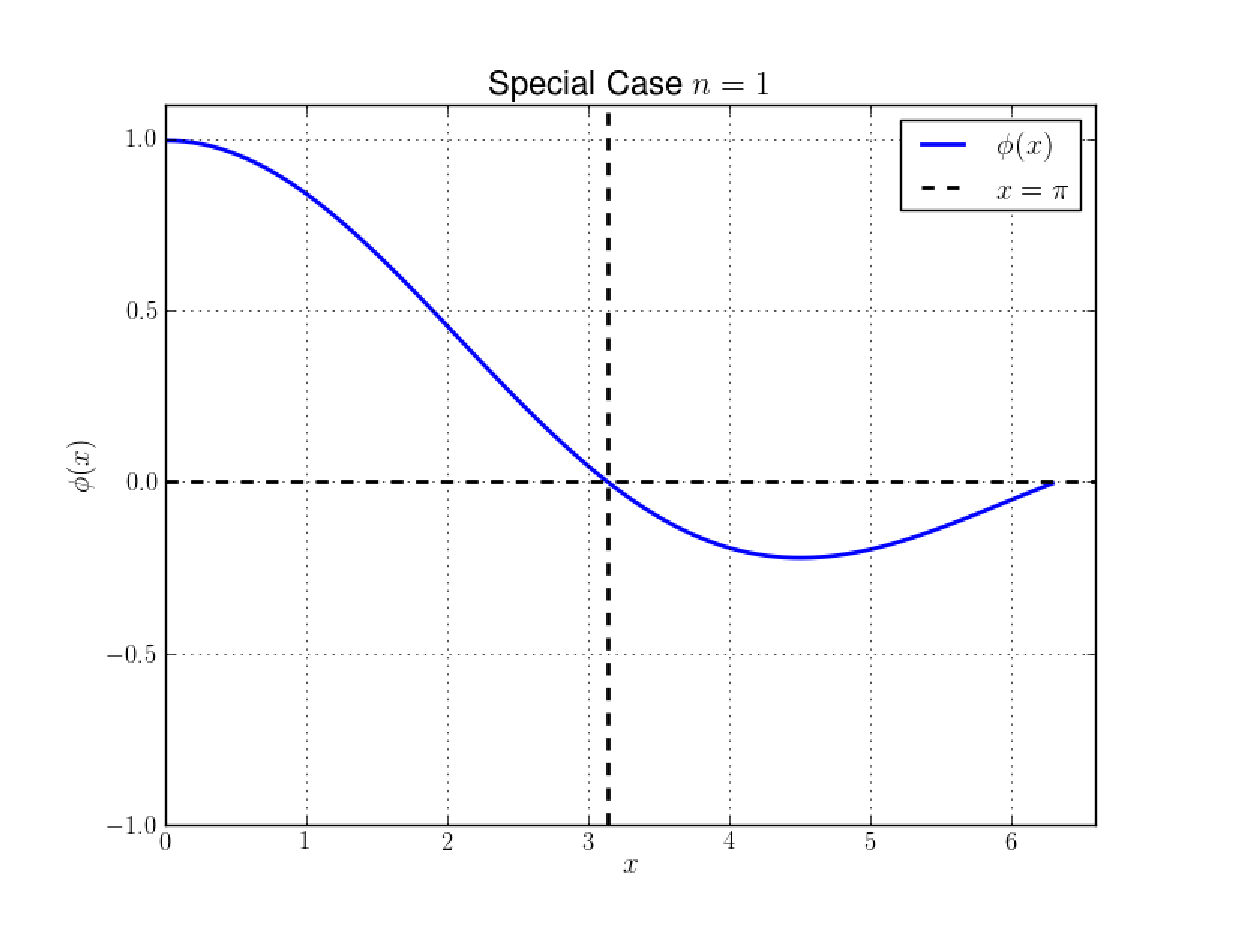
\includegraphics[scale=0.7]{images/LanEmdNeq1.eps}
  \caption{The solution to the Lane-Emden equation \eqref{eq:le}, for the special case of $n=1$. The surface of the star interpreted to be when $\phi(x)$ crosses the $x$-axis is at $x=\pi$ as shown in the figure.}\label{f:lnEmdN=1}
\end{center}
\end{figure}

Because our solution takes the analytical form shown in \eqref{eq:sinc} we see that $\phi(x)$ is zero whenever $x=n\pi$ where $n$ is any integer $\ge 1$. Thus the first time that $\phi$ crosses the $x$-axis is at $x=\pi$. Since $\rho = \lambda\phi^{n}$ (refer to \eqref{eq:theta})  this $x$-intercept is interpreted as the surface of the star due to the fact that at the surface the density is necessarily zero. Consequently, the range of physical interest for $\phi(x)$ is $0\le x\le\pi$.

The properties of this solution can be further uncovered by considering the gradient of the density\footnote{Essentially $\phi(x)$ in this case.} This is plotted on figure \eqref{f:grad}

\begin{figure}[h]
  \begin{center}
      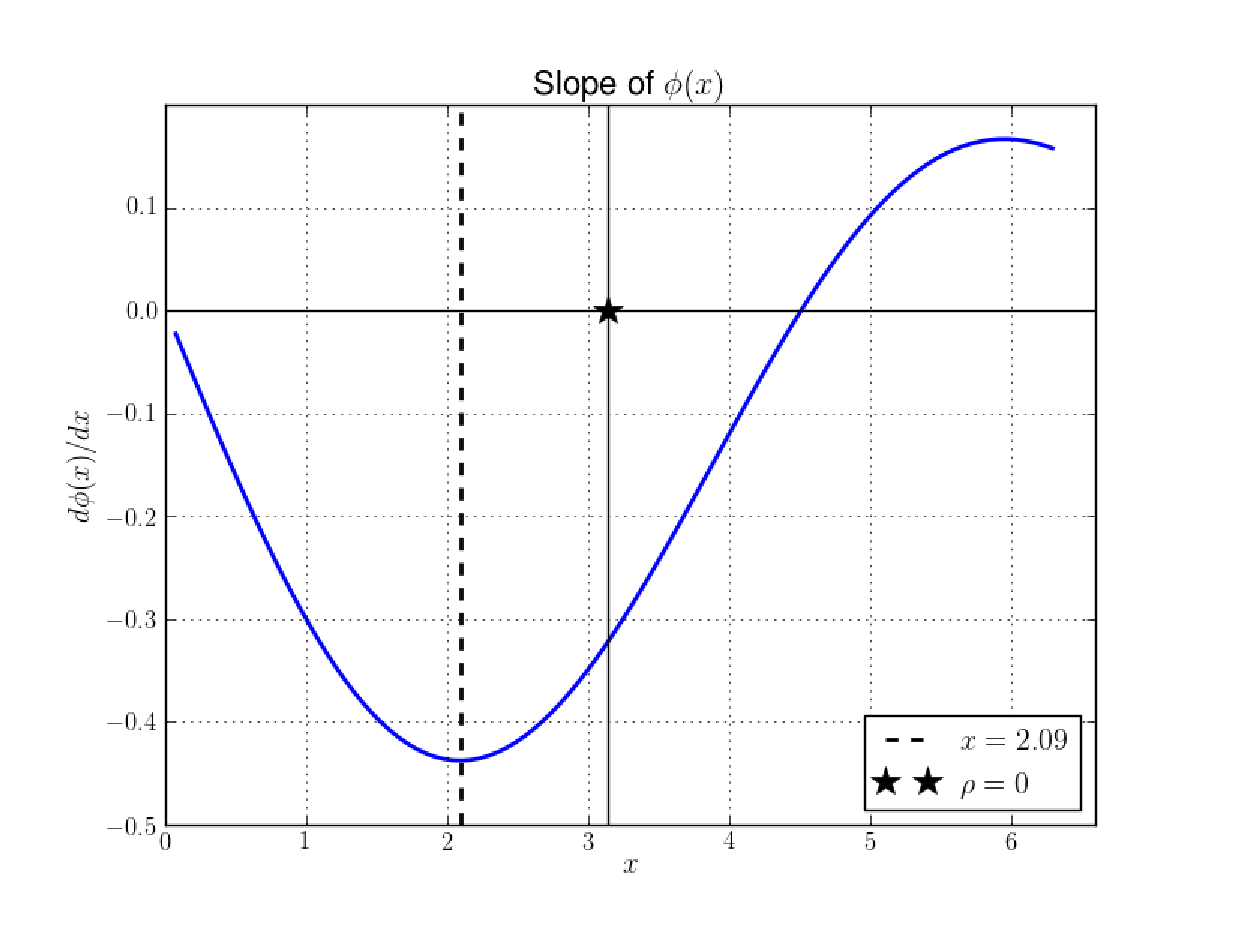
\includegraphics[scale=0.7]{images/SlopePhi.eps}\label{f:grad}
  \caption{The Gradient to the solution of the Lane-Emden \eqref{eq:le}, for the special case of $n=1$. The dotted line notes local minimum of this function at $x=2.09$ which denotes the position where the density of the star is changing the fastest.}
  \end{center}
  \end{figure}
The plot implies that the magnitude of the  gradient is greatest at $x=2.09$. However, one would expect that the gradient of the density be greatest near the center since gravity is a central force and goes as $1/x^{2}$. The closer one is to the center the greater the force to compact massive objects, this is compensated to some extent by the fact that the mass enclosed is less as one approaches the center. This effect could be explained by the requirement that the star be in hydrostatic-equilibrium as expressed in \eqref{eq:hydro}. Pressure has the tendency to want to disperse objects while gravity is constantly trying to bring them together. \par

Also unexpected is how abrupt the transition to zero density (i.e the surface) is. One would expect the transition to be asymptotic in nature. From figure \ref{f:grad} the rate of change in density at the surface is nowhere near zero. In fact it is $\approx75$\% of the maximum rate of change.

\section*{Solution for General $n$}
We attempt to find a series solution for $\phi \left( x \right)$ in the Lane-Emden equation for general $n$, where $n$ is a positive integer. Given the possibility of a singularity in the solution at $x = 0$, the Frobenius method allows us to write a series solution for $\phi \left( x \right)$ in identical form to Equation \eqref{eq:frbForm}, accounting for potential singularities (which, by physical constraints, should not exist). Then, by the Lane-Emden equation,

\begin{equation}
\sum_{k=0,even}^{\infty}a_k\left(k+p\right)\left(k+p-1\right)x^{k+p-2}+\sum_{k=0,even}^{\infty}a_k\left(k+p\right)x^{k+p-2}+\left[\sum_{k=0,even}^{\infty}a_kx^{k+p}\right]^n=0.\label{eq:genseries}
\end{equation}

Physical constraints necessitate that no negative powers of $x$ exist (as this would cause infinite densities at $x=0$); thus only non-negative values for p are possible. Since $p \geq 0$, the lowest power of the $\phi^n$ term in Equation \eqref{eq:genseries} will always be greater that those of the first two terms ($pn > p-2$). Thus our solution for p in general will match that found in the $n=1$ case, namely $p=0$.

Since $\phi\left(x\right)$ is an infinite-degree polynomial with a lowest power of zero, $\phi^n$ will likewise be an infinite-degree polynomial with lowest power zero. Therefore, a recursion relation can be found similar to that for the $n=1$ case, between $a_{k+2}$ and $a_{k}$. Furthermore, our general solution will contain only even or odd powers of $x$.

We can show that the purely even-powered solution is the appropriate choice for $\phi \left( x \right)$ in two ways. First and most straightforward is to point out that the first term of our series solutions from the Frobenius method was a constant (zeroth power) term, implying that each successive term must be even. Furthermore, we see also that this is physically appropriate because a constant term is needed for the density of the star at its center to not go to zero (which is an inevitability for a positively odd-powered solution).  

Once we have set the condition that the solution to the general Lane-Emden equation in $\phi \left( x \right)$ must contain only even powers of $x$, we can write the first three terms of the series solution to $\phi \left( x \right)$ as

\begin{equation}
\phi \left( x \right) = a_0 + a_2x^2 + a_4x^4 + \dots.
\end{equation}

Thus we have

%\begin{subequations}
\begin{align}
%\begin{equation}
\phi \left( x \right) = &\ a_0 + a_2x^2 + a_4x^4 + a_6x^6 + \dots \notag \\
\frac{d\phi}{dx} = &\ 2a_2x + 4a_4x^3 + 6a_6x^5 + \dots  \label{eq:lesf} \\
\frac{d^2\phi}{dx^2} =  &\ 2a_2 + 12a_4x^2 + 30a_6x^4 + \notag \dots
\end{align}
%\end{equation}
%\end{subequations}

and so the Lane-Emden equation \eqref{eq:lesf} can be written as

%\begin{equation}
\begin{align}\label{eq:gexseries}
\left[\left( 2a_2 + 12a_4x^2 + 30a_6x^4 + \dots \right)\right. &+ \notag \\
\left( 4a_2 + 8a_4x^2 + 12a_6x^4 + \dots \right) &+ \\
\left.\left( a_0 + a_2x^2 + a_4x^4 + \dots \right)^n\right] &= 0. \notag
\end{align}
%\end{equation}

In order to write $a_2$ and $a_4$ in terms of $a_0$, we must first consider the final term in Equation \eqref{eq:gexseries}, which is

\begin{equation}
\left( a_0 + a_2x^2 + a_4x^4 + \dots \right) \left( a_0 + a_2x^2 + a_4x^4 + \dots \right) \dots \text{n times}.
\end{equation}

We note that the only term in the resultant polynomial that is of zeroth order is that which is obtained by multiplying the $n\,a_0$ terms together. Therefore

\begin{equation}
2a_2 + 4a_2 + a_0^n = 0, \text{or} \notag
\end{equation}

\begin{equation}
a_2 = -\frac{a_0^n}{6}.
\end{equation}

For the $x^2$ terms we find that the only possible terms are those where one $a_2x^2$ term from one of the polynomials is multiplied by $n-1\,a_0$ terms in the remaining polynomials. There are $n\,a_2x^2$ terms, therefore

\begin{equation}
12a_4 + 8a_4 + na_0^{n-1}a_2 = 0, \text{or} \notag
\end{equation}

\begin{equation}
a_4 = \frac{na_0^{2n-1}}{120}.
\end{equation}

The first three terms can then be written for general n:

\begin{equation}
\phi \left( x \right) = a_0 - \frac{a_0^n}{6}x^2 + \frac{na_0^{2n-1}}{120}x^4 + \dots.
\end{equation}

If we set $n=1$ and compare our result to the first three terms of the analytic solution for $n=1$ which are

\begin{equation}
\phi \left( x \right) = a_0 \left(1 - \frac{x^2}{3!} + \frac{x^4}{5!} + \dots \right)
\end{equation}

we find that the terms agree.

\section*{Numerical Solutions for $n = 2$}
    The Runge-Kutta method (RK4) is an effective numerical tool for finding a solution to a given differential equation. It works by making four successive approximations to the solution around the starting point, $x_{0}$, defined by the initial conditions of the problem.
    The motivation behind the RK4 method consists of finding the appropriate constants such that 
    \begin{equation}
        y_{n+1} = y_n + a\eta_1 + b\eta_2 + c\eta_3 + d\eta_4
    \end{equation}
    agrees with a Taylor series expansion up to the fifth term, or out to $4^{\text{\tiny{th}}}$ order \cite{zill}. To find $y_{n+1}$ from $y_n$, we evaluate four successive slopes of $f(x, y)$ given by
    \begin{equation}
        y' = f(x, y)
    \end{equation}
    and take a weighted average. In order, we follow the following prescription \cite{blanch} for evaluating the four slopes given a step-size $h$:
    \begin{enumerate}
        \item
            At position $(x_0, y_0)$, the slope is 
            \begin{equation}\label{eq:slope1}
                \eta_1 = f(x_0, y_0)
            \end{equation}
        \item
            The $x$-coordinate is incremented by $h/2$ so that the next $y$-coordinate is 
            \begin{equation}
                y_1 = y_0 + \eta_1\frac{h}{2}
            \end{equation}
            and the second slope is then 
            \begin{equation}\label{eq:slope2}
                \eta_2 = f(x_0 + h/2, y_1)
            \end{equation}
        \item
            Using the same $x$-position, we find another $y$-coordinate using the slope we previously calculated, $\eta_2$
            \begin{equation}
                y_3 = y_0 + \eta_2\frac{h}{2}
            \end{equation}
            to the get the next successive slope
            \begin{equation}\label{eq:slope3}
                \eta_3 = f(x_0 + h/2, y_3)
            \end{equation}
        \item
            The last slope is obtained at the position $x = x_0 + h$, where again we use our previously calculated slope $\eta_3$ to determine the corresponding $y$-coordinate,
            \begin{equation}
                y_4 = y_0 + \eta_3h
            \end{equation}
            and the slope at that position is
            \begin{equation}\label{eq:slope4}
                \eta_4 = f(x_0 + h, y_4)
            \end{equation}
    \end{enumerate}
        The slopes at the midpoint ($x+h/2$) are weighted twice as much as the other two slopes in the averaging and the successive solution of $y$ is then
            \begin{equation}
                y_{n+1} = y_n + \left(\eta_1+2\eta_2+2\eta_3+\eta4\right)\frac{h}{6}.
            \end{equation}
   

    Because the RK4 method works best for $1^{\text{\tiny{st}}}$-order differential equations, and since we wish to find a numerical solution to a $2^{\text{\tiny{nd}}}$-order differential equation, we need to add an addition adjustment to our algorithm. The Lane-Emden equation of $n = 2$ can be written as 
    \begin{equation}\label{eq:phinl}
        \phi'' + \frac{2}{x}\phi' + \phi^2 = 0
    \end{equation} 
    which can be reduced to two $1^{\text{\tiny{st}}}$-order differential equations.  First, we assign 
        \begin{equation}
            v = \phi' = f(x, y, v)
        \end{equation}
        and then \eqref{eq:phinl} becomes
        \begin{equation}
            v' = - \frac{2}{x}v - \phi^2 = g(x, y, v)
        \end{equation}
        To solve \eqref{eq:phinl}, we must now evaluate the increments of $\phi$ and $v$ with the following updated recipe \cite{lea} for finding the slopes:
        \begin{align}
            \eta_1 =& hf(x_0, y_0, v_0) \notag \\ 
            m_1 =& hg(x_0, y_0, v_0)\notag \\ 
            \eta_2 =& hf(x_0 + h/2, y_0 + \eta_1/2, v_0 + m_1/2)\notag \\
            m_2 =& hg(x_0+h/2, y_0 + \eta_1/2, v_0 + m_1/2) \notag\\
            \eta_3 =& hf(x_0 + h/2, y_0 + \eta_2/2, v_0 + m_2/2) \label{eq:algor}\\
            m_3 =& hg(x_0+h/2, y_0 + \eta_2/2, v_0 + m_2/2) \notag \\
            \eta_4 =& hf(x_0 + h, y_0 + \eta_3, v_0 + m_3) \notag\\
            m_4 =& hg(x_0+h, y_0 + \eta_3, v_0 + m_3)\notag\\ \notag
        \end{align}
        Just as $y$ is incremented by the averaged $\eta$, $v$ is incremented by the similarly averaged $m$.

    As a sanity check, we plotted the numerical solution of the Lane-Emden equation for the case of $n = 1$ and checked the result against our series solution found earlier. We find that for a step-size of $h = 0.1$, the numerical solution agrees with our series solution and we may proceed further to the case of $n = 2$.
    \begin{figure}[H]
        \begin{center}
            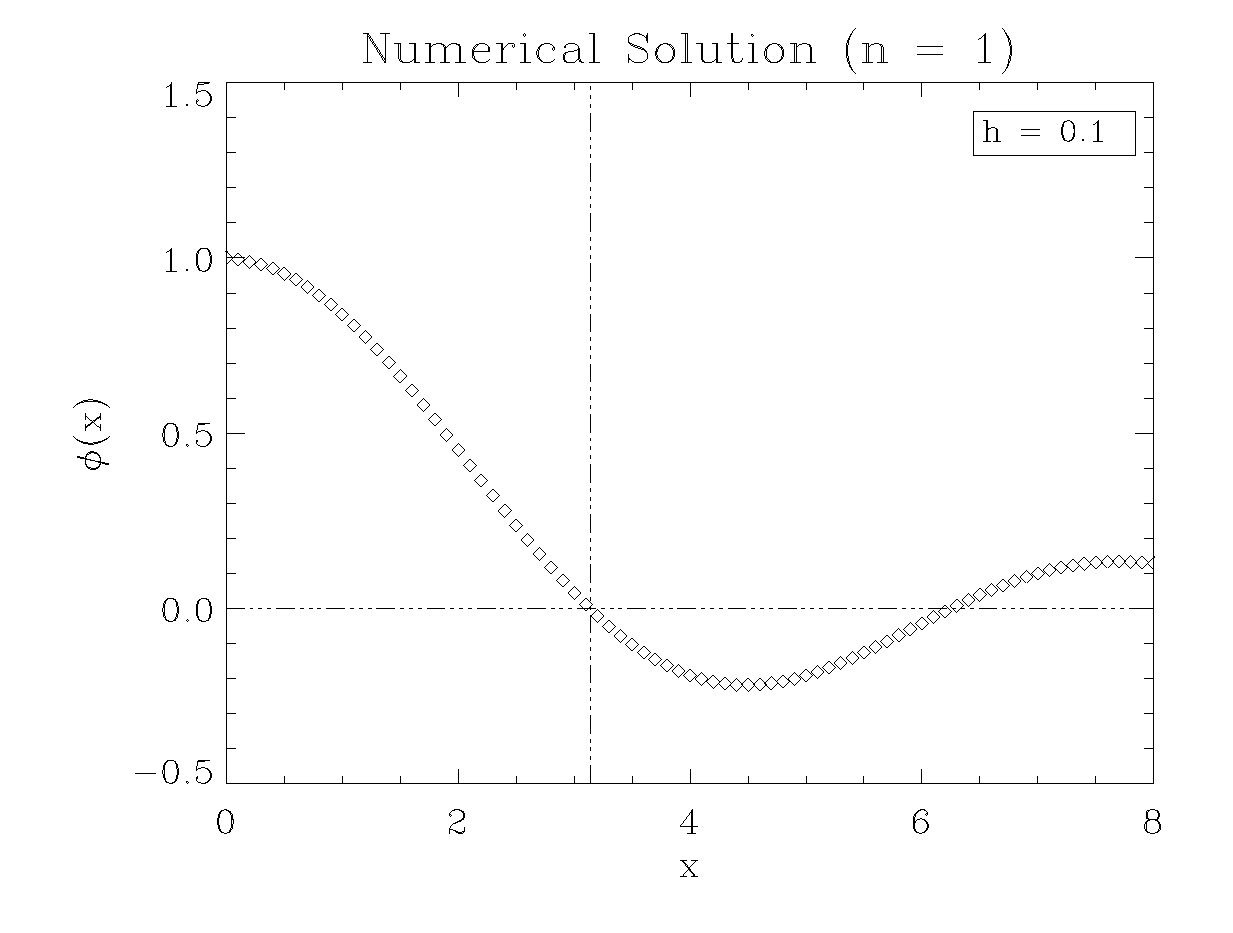
\includegraphics[scale=0.58]{images/rk4plotn1.eps}
            \caption{The numerical solution of the Lane-Emden equation of polytropic index $n = 1$.}
            \label{fig:numplot2}
        \end{center}
    \end{figure}

  %  Based on the algorithm described by \eqref{eq:algor}, we wrote a procedure in IDL (Appendix B) in order to generate an array of solutions for the Lane-Emden equation for $n = 2$ and plotted our results in figure \eqref{fig:numplot1} for three different step-sizes. We notice that for $h = 0.5$, our solutions for $\phi(x)$ diverge slightly from both the other smaller step-sizes, which appear to produce almost identical results. 
    \begin{figure}[H]
        \begin{center}
            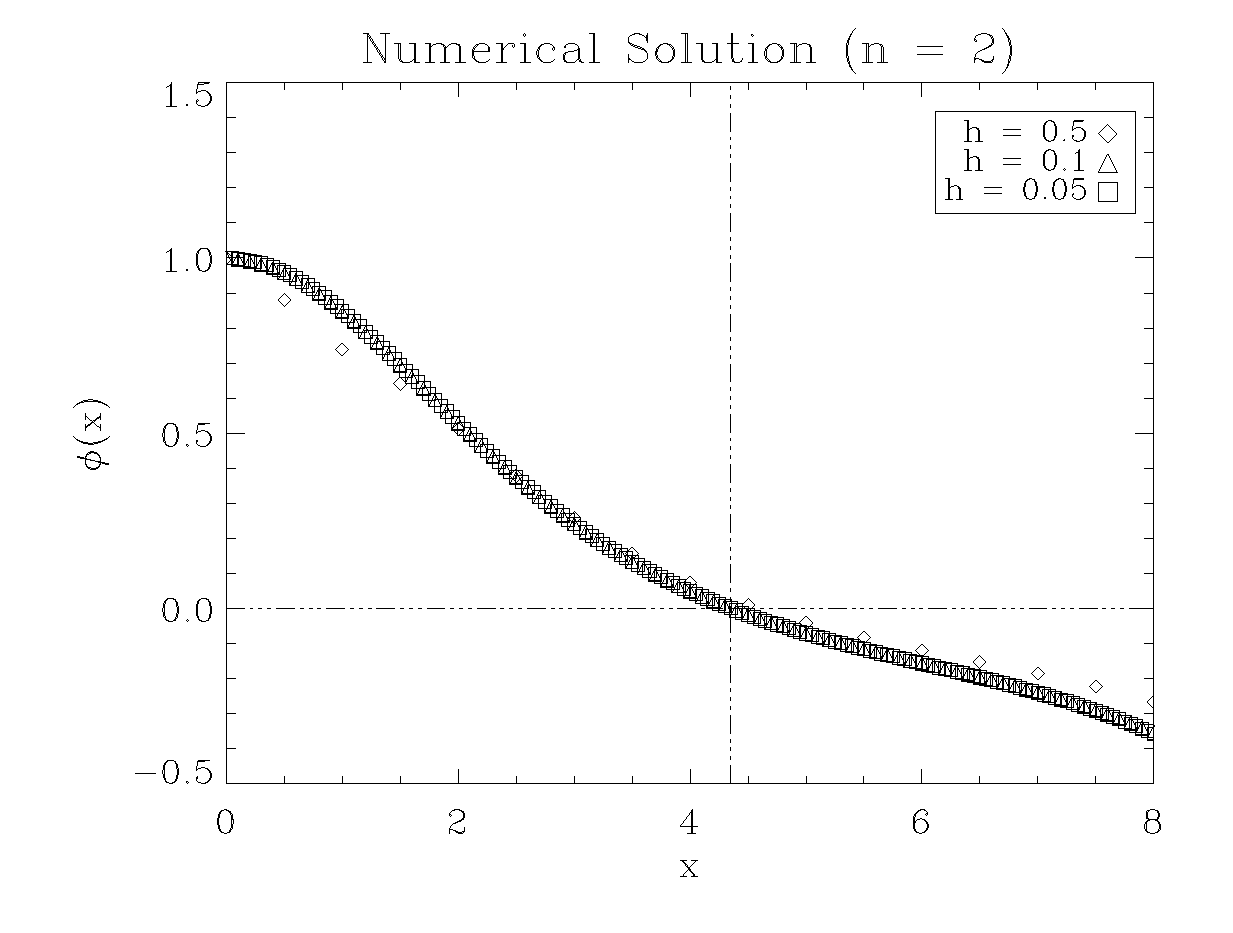
\includegraphics[scale=0.58]{images/rk4plot.eps}
            \caption{The numerical solutions for $n = 2$ using the RK4 method for three different step sizes are shown. The solutions intersect the $x$-axis at $\sim$ 4.35. The value of the dimensionless distance where $\phi(x) = 0$ corresponds to the radius of the star.}
            \label{fig:numplot1}
        \end{center}
    \end{figure}
    Based on the algorithm described by \eqref{eq:algor}, we wrote a procedure in IDL (Appendix B) in order to generate an array of solutions for the Lane-Emden equation for $n = 2$ and plotted our results in figure \eqref{fig:numplot1} for three different step-sizes. We notice that for $h = 0.5$, our solutions for $\phi(x)$ diverge slightly from both the other smaller step-sizes, which appear to produce almost identical results. 

To get a sense of how our numerical solutions vary with step-size, we evaluated $\phi(x = 1)$ for the case of $n = 1$ for a range of $h$ and plotted the results in figure \eqref{fig:diffn1}. We notice that the output converges rapidly with smaller and smaller step-sizes. However, once we choose $h = 0.1$, we can expect approximately the same precision as $h = 0.001$. According to table \eqref{tab:diff}, once $h$ is smaller than $0.1$, the percent difference between subsequent dimishing step-sizes begins to oscillate toward zero at the cost of computing time with minor improvement. 
\begin{figure}[H]
    \begin{center}
        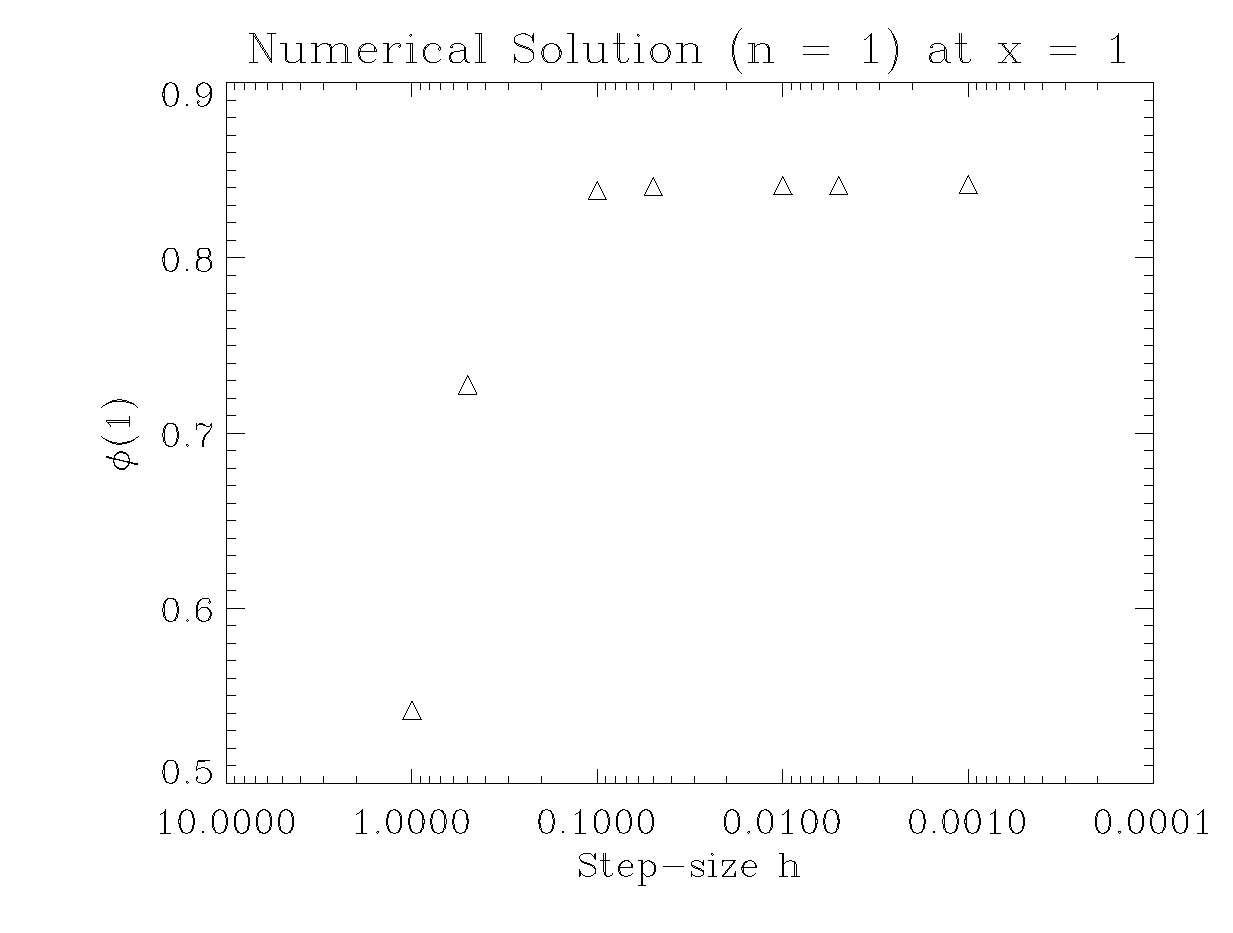
\includegraphics[scale=0.6]{images/diffn1.eps}
        \caption{The figure shows $\phi(1)$ evaluated with varying step-size $h$.}\label{fig:diffn1}
    \end{center}
\end{figure}
\input{images/diff.txt}

After comparing our RK4 solution against the $n = 1$ series solution and choosing an appropriate step-size, we are confident in our result for the solutions to the case of $n = 2$. We can now make a comparison between our approximate three term series solution for arbitrary $n$ and our RK4 method. Figure \eqref{fig:3term} depicts the case for $n = 1$. We can see that up to $x \simeq 2$, the two solutions agree but diverge significantly thereafter. We can image that finding more than three terms in our series solution would produce a result that would agree more closely with our RK4 solution.
\begin{figure}[H]
    \begin{center}
        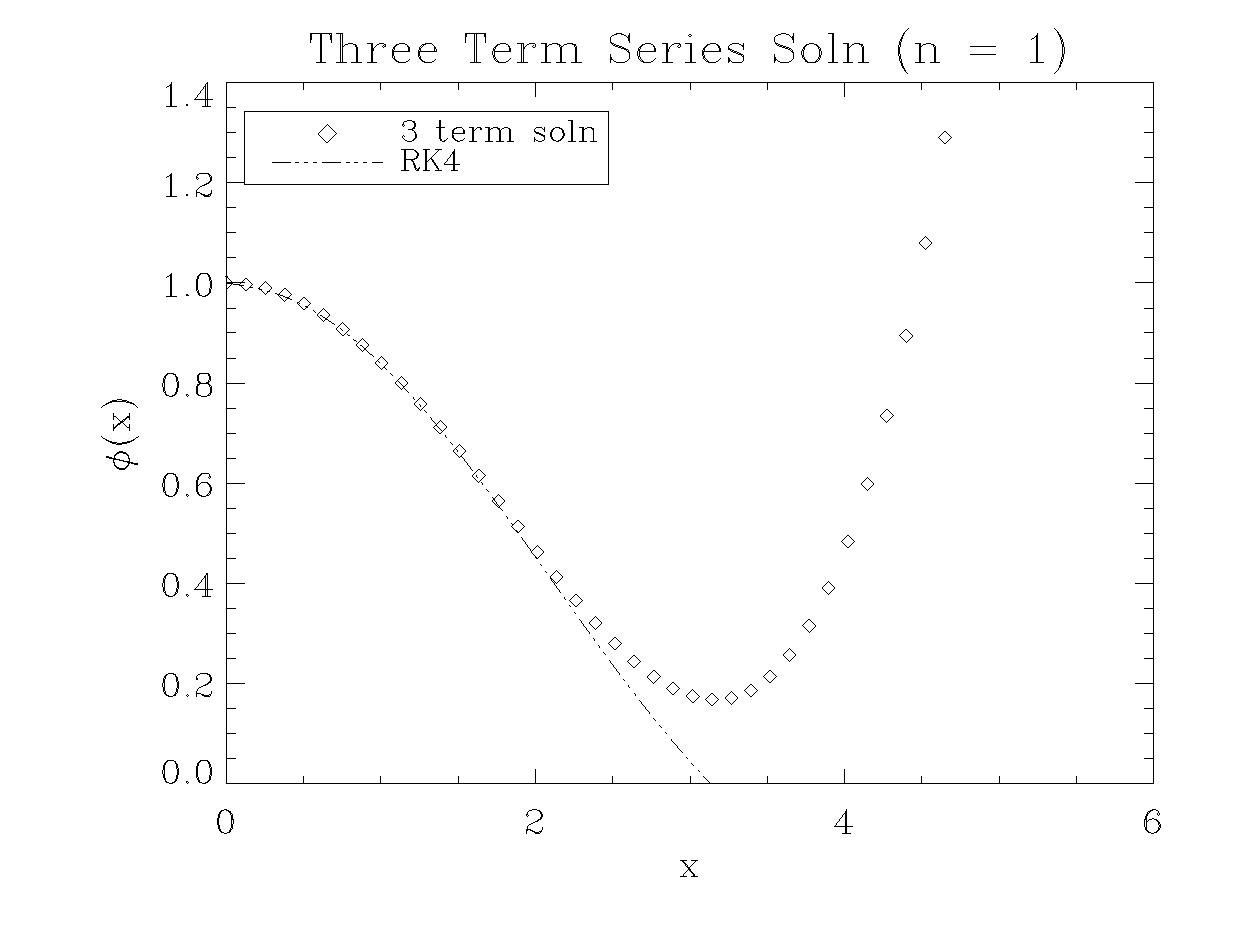
\includegraphics[scale=0.6]{images/3term_n1.eps}
        \caption{A comparison between the first three terms to our solution for an arbitrary $n$ (setting $n = 1$, here) and the RK4 method for the case of $n = 1$ is depicted in this plot. We notice that the two solutions begin to diverge at around $x = 2$.}\label{fig:3term}
    \end{center}
\end{figure}

\section*{Conclusion}
We have shown that for $n = 1$, the Lane-Emden equation can produce an analytic solution of $\text{sinc}x$. This solution is zero for when the dimensionless quantity $x$ is $\simeq 3.14$ which puts a contraint on the radius of the star we are modeling. When considering the case of an arbitrary polytropic index, we discovered that finding the first three terms of the series solution did not produce results that matched well to our numerical solution for $n = 1$, and that to improve accuracy, we needed to define the series solutions with more than three terms. Finally, when we considered our numerical solution for $n = 2$, we found that while decreasing the step-size $h$ allowed the solution to converge, that no real gain was made by any further decrease in $h$ below $h = 0.1$.
\begin{appendices}
\section{Result Tables RK4 Method}
\input{images/rk4letable.txt}
\input{images/rk4letable2.txt}

\section{Source Code}
\begin{verbatin}

\end{verbatim}
\begin{verbatim}
    FUNCTION rk4le, h, N
    ;+
    ; NAME: rk4le
    ;
    ; PURPOSE: 
    ;   Iteratively solves a first order differential equation
    ;       using the 4th-order Runge-Kutta method. 
    ;
    ; EXPLANATION:
    ;   This procedure calls on two functions which are the constituent
    ;       pieces of a 2nd-order differential equation. For example, if 
    ;       y'' + y' = 0, then v = y' is our first constituent, and 
    ;       v' + v = 0 is our second constituent, and this procedure works
    ;       to solve both pieces.
    ;
    ; CALLING SEQUENCE:
    ;   xymatrix = rk4le(h, N)
    ;
    ; INPUTS:
    ;   h - step-size per interation
    ;   N - numbers of interations
    ;
    ; OUTPUTS:
    ;   Returns a 2 by N dimensional matrix containing the solution and its
    ;       independent variable.
    ;
    ; EXAMPLE:
    ;   IDL> xy = rk4le(0.1, 100.)
    ;   IDL> x = xy[*,0]
    ;   IDL> y = xy[*,1]
    ;
    ; RESTRICTIONS:
    ;   This procedure was designed to cater to solving the Lane-Emden 
    ;       equation and initial conditions are currently hardcoded in. 
    ;       MOre generality will come in the future.
    ; PROCEDURES CALLED:
    ;   None
    ;
    ; REVISION HISTORY:
    ;   Written by Adam Fries, Allan Gamboa, and Arthur Adams
    ;       Oct 2012 based off of 'Mathematics for Physicists'
    ;       by Susan M. Lea pgs. 202-205
    ;-

    ;; set up Lane-Emden initial conditions
    x0 = 0.000000000000000000001
    y0 = 1
    v0 = 0.

    ;; save IC values
    y = y0
    x = x0

    ;; loop through and find each solution per incremented x0
    for i  = 0L, N - 1 do begin
        k1 = h*myf2(x0, y0, v0)
        m1 = h*myg2(x0, y0, v0)
        k2 = h*myf2(x0 + 0.5*h, y0 + 0.5*k1, v0 + 0.5*m1)
        m2 = h*myg2(x0 + 0.5*h, y0 + 0.5*k1, v0 + 0.5*m1)
        k3 = h*myf2(x0 + 0.5*h, y0 + 0.5*k2, v0 + 0.5*m2)
        m3 = h*myg2(x0 + 0.5*h, y0 + 0.5*k2, v0 + 0.5*m2)
        k4 = h*myf2(x0 + h, y0 + k3, v0 + m3)
        m4 = h*myg2(x0 + h, y0 + k3, v0 + m3)
       
        ;; add adjustments
        x0 += h
        y0 += (k1 + 2.*k2 + 2.*k3 + k4)/6.
        v0 += (m1 + 2.*m1 + 2.*m3 + m4)/6.
        
        ;; catenate solutions
        x = [x, x0]
        y = [y, y0]
    endfor

    ;; return solution as a matrix
    return, [[x],[y]]

    end

    FUNCTION myf2, x, y, v
    ;;       y' = f(x,y,v) = v
    f = v
    return, f
    end

    FUNCTION myg2, x, y, v
    ;;       v' = g( x, y, v) = -y^2 - 2v/x
    g = -y^2. - 2.*v/x
    return, g
    end

    
    PRO learb_n, n
    ;;
    ;; This code was created to plot the 3 term  series
    ;;  solution against our RK4 solution for n = 1
    ;;
    x = findgen(100)/100*4*!pi
    a0 = 1.

    phi = a0*(1. - (a0^n)/6.*x^2. + n*a0^(2.*n - 1.)/120.*x^4.)

    phir = rk4le(0.1, 100)

    title = '!6Three Term Series Soln (n = 1)'
    xtitle = '!6x'
    ytitle = '!7u!6(x)'
    plot, x, phi, charsize = 1.6, psym = 4, yr = [0, 1.25], xr = [0,6] $
        , title = title, xtitle = xtitle, ytitle = ytitle
    oplot, phir[*,0], phir[*,1], line = 4
    legend, ['!63 term soln', 'RK4'], psym = [4,0], line = [0,4] $
        , charsize = 1.4

    end


\end{verbatim}
\end{appendices}
\bibliographystyle{plain}
\bibliography{laneemden.bib}
\end{document}
